\documentclass{article}
\usepackage{graphicx}
\usepackage{epstopdf, epsfig}
\usepackage{newtxtext}
\usepackage{newtxmath}
\usepackage{hyperref}
\usepackage{color}
\usepackage{siunitx}
\usepackage[square, numbers]{natbib}
\title{Supplementary Information for `Asymptotic Analysis of Subglacial Plumes in Stratified Environments` by Bradley et al.}
\author{Alexander T Bradley, C. Rosie Williams, \\ Adrian Jenkins, Robert Arthern}
\date{}
\begin{document}
\maketitle
\newcommand{\Pb}{\textit{P}_B}  %\frac{L/c}{ \tau}\frac{S_l - S_u}{2S_l},
\newcommand{\lt}{\delta} %dimensionless thermocline length, lt/l0
\newcommand{\Pt}{\textit{P}_T}
\renewcommand{\in}{\text{in}} %subcript on into and out of pycnocline variables
\newcommand{\out}{\text{out}}
\newcommand{\order}[1]{\mathcal{O}(#1)}
 \newcommand{\dd}[2]{\frac{\mathrm{d} #1}{\mathrm{d} #2}}
 \newcommand{\epsone}{\epsilon_1}

In this supplementary information we provides further details on the analysis presented in the main text. This suppelementary consists of five sections: in the first, We explicitly state the solution in region one and associated matching conditions for region two; in the second, we explicitly state the pycnocline-rescaled plume model equations; in the third, we provide details of the behaviour of solutions in region three in the limit $X \to X_c$; in the fourth section we provide further details of the behaviour in region 4; finally, we explicitly state our constructed melt rate parametrizations in special cases discussed in \S4 of the main text.

\section{Solution for Region One and Matching Conditions on Region Two}
The solution to the leading order equations appropriate for region one, given by (3.1)--(3.4) in the main text, is:
\begin{align}
U(X) &=\left(\frac{2\kappa}{3}\right)^{1/2}\left[Z_b'(X)\right]^{1/3}\left[1 - Z_b(X)\right]^{1/3}I(X)^{1/2},\\
%D &= \frac{2}{3}\left[Z_b'(X)\right]^{-1/3}\left[1 - Z_b(X)\right]^{-1/3}I(X),\label{E:Region1:thickness_solution}\\
D(X) &= \frac{2}{3}\left[Z_b'(X)\right]^{-1/3}\left[1 - Z_b(X)\right]^{-1/3}I(X),\label{E:Region1:thickness_solution}\\
\Delta \rho(X) &= \kappa \left[ 1- Z_b(X)\right],\label{E:Region1:buoyancy_solution}\\
%\Delta T &= Z_b'(X)\left[1 - Z_b(X)\right]\left\{1 - %\frac{2}{3}I(X)\left[Z_b'(X)\right]^{1/3}\left[1-Z_b(X)\right]^{-4/3}\right\}
\Delta T &= \left[1-Z_b(X)\right]Z_b'(X) - \frac{2}{3}\left[Z_b'(X)\right]^{2/3} \left[1-Z_b(X)\right]^{-1/3}I(X),\label{E:Region1:thermal_solution}
\end{align}
where
\begin{equation}
I(X) =  \int_0^X \left[Z_b'(\xi)\right]^{4/3}\left[1 - Z_b(\xi)\right]^{1/3}~\mathrm{d}\xi.
\end{equation}
The matching conditions on region two are therefore given by
\begin{align}
U \to U_\text{in} &=\left(\frac{2\kappa}{3}\right)^{1/2}\left[Z_b'(X_p)\right]^{1/3}\left[1 - Z_b(X_p)\right]^{1/3}I(X)^{1/2},\\
%D &= \frac{2}{3}\left[Z_b'(X)\right]^{-1/3}\left[1 - Z_b(X)\right]^{-1/3}I(X),\label{E:Region1:thickness_solution}\\
D \to D_\text{in} &= \frac{2}{3}\left[Z_b'(X_p)\right]^{-1/3}\left[1 - Z_b(X_p)\right]^{-1/3}I(X_p),\label{E:Region1:thickness_solution}\\
\Delta \rho \to \Delta \rho_\text{in} &= \kappa \left[ 1- Z_b(X_p)\right],\label{E:Region1:buoyancy_solution}\\
%\Delta T &= Z_b'(X)\left[1 - Z_b(X)\right]\left\{1 - %\frac{2}{3}I(X)\left[Z_b'(X)\right]^{1/3}\left[1-Z_b(X)\right]^{-4/3}\right\}
\Delta T \to \Delta T_{\text{in}} &= \left[1-Z_b(X_p)\right]Z_b'(X_p) - \frac{2}{3}\left[Z_b'(X)\right]^{2/3} \left[1-Z_b(X)\right]^{-1/3}I(X),
\end{align}
as $\zeta = (X - X_p)/\delta \to -\infty$.

\section{Pycnocline-rescaled plume model equations}
The pycnocline-rescaled plume model equations referred to in \S3.2 in the main text read:
\begin{align}
\dd{(DU)}{\zeta} &=\lt U Z_b'(X_p + \lt \zeta) + k_3 \epsone \lt U \Delta T,		\label{E:PycnoclineRegion:MassFull}	\\
\cone \dd{(DU^2)}{\zeta} &=  D\Delta \rho Z_b'(X_p + \lt \zeta)  -  U^2,	\label{E:PycnoclineRegion:MomFull}	\\
\dd{(DU\Delta \rho)}{\zeta} &= -\Pb \mathrm{sech}^2(\zeta)Z_b'(X_p + \lt \zeta)DU + \lt \left[\kappa - k_4 \epsone \tanh(\zeta)\right] U \Delta T \label{E:PycnoclineRegion:BuoyancyFull}		\\
\ctwo \dd{(DU\Delta T)}{\zeta} &= \left\{1 - Z_b(X_p + \lt \zeta) - \Pt\left[1 + \tanh(\zeta)\right] - D\right\}UZ_b'(X_p + \lt \zeta) -U\Delta T.\label{E:PycnoclineRegion:ThermalFull}
\end{align}

%%%%%%%%%%%%%%%%%%%%%% Analysis of Region 3 as X \to X_c %%%%%%%%%%%%
\section{Analysis of Region Three in the Limit $X \to X_c$}
In this section, we describe the behaviour of solutions of the leading order equations for region three in the limit $X \to X_c$, where the velocity $U$ approaches zero. Recall that these leading order equations are 
\begin{align}
 (DU)' &= U Z_b', \label{E:Region3:mass} \\
0 &= D \Delta \rho Z_b' - U^2, \label{E:Region3:mom}\\
(DU\Delta \rho)'  &=\kappa U \Delta T  \label{E:Region3:buoyancy}\\
0&= (1  - 2\Pt -  Z_b)Z_b'U- U\Delta T - DU Z_b',\label{E:Region3:thermal}
\end{align}
and that the flux $Q = DU$ evolves according to
\begin{equation}\label{E:Region3:Q_ODE}
%\left(Q'\right)^3 =\kappa \left(Z_b'\right)^4 \left\{\left(1 - Z_b\right)Q - 2\Pt\left(Q - Q_\in\right) -\left[1 - Z_b(X_p)\right]Q_\in\right\} + \frac{U_\out^3}{Z_b'(X_p)}\left(Z_b'\right)^4.
\frac{\left[Q'(X)\right]^3}{\left[Z_b'(X)\right]^4} = \kappa \left\{ \left[1 - Z_b(X) - 2P_T\right] Q(X) - \left[1 - Z_b(X_p) - 2P_T\right]Q_\text{in}\right\} + \frac{U_\text{out}^3}{Z_b'(X_p)}.
\end{equation}
The point $X_c$ satisfies 
\begin{equation}
\left[1 - Z_b(X_c)\right]Q_c - 2\Pt\left(Q_c - Q_\in\right) -\left[1 - Z_b(X_p)\right]Q_\in +  \frac{U_\out^3}{\kappa Z_b'(X_p)} = 0.
\end{equation}
where $Q_c = Q(X_c)$.

Since the velocity $U \to 0$ as $X = X_c$, we must introduce rescaled variables to reflect a change in asymptotic order; we therefore introduce
%\begin{align}
%U &\sim \kappa^{1/3} Z_b'(X_c)^{2/3} Q_c^{1/3}(X_c - X)^{1/3}, & D &\sim \kappa^{-1/3} Z_b'(X_c)^{-2/3} Q_c^{2/3}(X_c - X)^{-1/3},\label{E:Region3:X_to_Xc1}\\
%\Delta \rho &\sim  \kappa Z_b'(X_c) (X_c - X), & \Delta T &\sim -\kappa^{-1/3} Z_b'(X_c)^{1/3} Q_c^{2/3}(X_c - X)^{-1/3}\label{E:Region3:X_to_Xc2}
%\end{align}
\begin{equation}\label{E:Region3:Rescaling}
X = X_c + \varepsilon \tilde{X}, \quad Q = Q_c + \varepsilon^\gamma \tilde{Q}
\end{equation}
where $\varepsilon \ll 1$ is arbitrary, $\tilde{X} =\order{1}$ is negative, $\tilde{Q} = \order{1}$ and $\gamma >0$ is to be determined. Inserting~\eqref{E:Region3:Rescaling} into~\eqref{E:Region3:Q_ODE} gives
\begin{multline}\label{E:Region3:RescaledODE}
\varepsilon^{3(\gamma - 1)}\frac{\left(\tilde{Q'}\right)^3}{\left[Z_b'(X_c)\right]^4}\left[1 + \order{\varepsilon} \right]= -\varepsilon\lambda\tilde{X}Z_b'(X_c)Q_c + \\ \varepsilon^\gamma \left[1 - 2\Pt - Z_b(X_c)\right] \tilde{Q} + \order{\varepsilon^2, \varepsilon^{\gamma + 1}}.
\end{multline}
A dominant balance is obtained in~\eqref{E:Region3:RescaledODE} by taking $\gamma = 4/3$. After setting $\gamma = 4/3$ in~\eqref{E:Region3:RescaledODE}, using $Q' = U Z_b'$ [from~\eqref{E:Region3:mass}] and undoing the rescaling~\eqref{E:Region3:Rescaling}, we find 
\begin{equation}\label{E:Region3:U_asym}
U \sim \kappa^{1/3} Z_b'(X_c)^{2/3} Q_c^{1/3}(X_c - X)^{1/3} \quad \text{as}~X \to X_c^-.
\end{equation}
From~\eqref{E:Region3:Rescaling}, we have $Q \sim Q_c + \order{\varepsilon^{4/3}}$. Combining this with~\eqref{E:Region3:mass} gives
\begin{equation}\label{E:Region3:D_asym}
D \sim \kappa^{-1/3} Z_b'(X_c)^{-2/3} Q_c^{2/3}(X_c - X)^{-1/3} \quad \text{as}~X \to X_c^-.
\end{equation}
A balance in the momentum equation~\eqref{E:Region3:mom} gives
\begin{equation}\label{E:Region3:drho_asym}
\Delta \rho \sim  \kappa Z_b'(X_c) (X_c - X)\quad \text{as}~X \to X_c^-,
\end{equation}
while a balance in the thermal driving equation~\eqref{E:Region3:thermal} requires
\begin{equation}\label{E:Region3:dT_asym}
 \Delta T \sim -\kappa^{-1/3} Z_b'(X_c)^{1/3} Q_c^{2/3}(X_c - X)^{-1/3} \quad \text{as}~X \to X_c^-.
 \end{equation}

\section{Further Details of Region Four Behaviour}
%scaled variables for this region
\newcommand{\U}{\mathcal{U}}
\newcommand{\D}{\mathcal{D}}
\newcommand{\p}{\Delta \varrho}
\renewcommand{\t}{\Delta \mathcal{T}}
In this section, we provide further details of the behaviour of the leading order equations in region four. Recall that these equations are 
\begin{align}
\dd{(\D\U)}{\chi} &=0, &
\dd{(\D \U^2)}{\chi} &=  \D \p Z_b'(X_c) -\U^2,\label{E:Region4:mass_scaled}\\
\dd{(\D\U\p)}{\chi} &=\kappa  \U\t, &
k_2 \dd{(\D \U \t)}{\chi} &=- \U \t - \D \U Z_b'(X_c).\label{E:Region4:thermal_scaled}
\end{align}
for $ \chi > -\infty$. Equations~\eqref{E:Region4:mass_scaled}--\eqref{E:Region4:thermal_scaled} must satisfy the matching conditions
\begin{align}
\U &\sim \kappa^{1/3}Z_b'(X_c)^{-2/3}Q_c^{1/3} (-\chi)^{1/3}, &  \D &\sim \kappa^{-1/3} Z_b'(X_c)^{-2/3} Q_c^{2/3}(-\chi)^{-1/3}\label{E:Region4:far_field1},\\
\p &\sim - \kappa Z_b'(X_c) \chi, & \t &\sim -\kappa^{-1/3} Z_b'(X_c)^{1/3} Q_c^{2/3}(-\chi)^{-1/3}\label{E:Region4:far_field2}.
\end{align}

We begin by nothing that from the first of~\eqref{E:Region4:mass_scaled}, flux is conserved, i.e.
\begin{equation}\label{E:Region4:Constant_Flux}
    \D \U  = Q_c.
\end{equation}
Also, after inserting~\eqref{E:Region4:Constant_Flux} into the second of~\eqref{E:Region4:thermal_scaled}, we obtain an expression that  can be directly integrated to give
\begin{equation}\label{E:Region4:Linear_p_t}
    \frac{\p}{\kappa} + k_2 \t = -Z_b'(X_c) + C,
\end{equation}
where $C$ is a constant that would be determined by analysing the higher order contributions to $\Delta \rho$ as $X \to X_c$. This higher order analysis is beyond the scope of this paper.

The relationships~\eqref{E:Region4:Constant_Flux} and~\eqref{E:Region4:Linear_p_t} allow us to reduce~\eqref{E:Region4:mass_scaled}--\eqref{E:Region4:thermal_scaled} to a system of two equations, which can be rescaled so that only a single parameter, $k_2$, enters:
\begin{equation}\label{E:Region4:rescaled}
\tilde{\U} \dd{\tilde{\U}}{\tilde{\chi}} = \tilde{\p} - \tilde{\U}^3, \qquad 
k_2  \dd{\tilde{\p}}{\tilde{\chi}} = -\tilde{\U}\left[\tilde{p} + \tilde{\chi}\right],
\end{equation}
where
\begin{align}
\tilde{\chi} &= \frac{\kappa^{1/4}Z_b'(X_c)^{1/2}}{Q_c^{1/2}}\left(\chi - \frac{C}{\kappa Z_b'(X_c)}\right), \label{E:Region4:RescalingChi} \\ 
\tilde{\U} &= \frac{1}{\kappa^{1/4}Z_b'(X_c)^{1/2}Q_c^{1/2}}\U, \label{E:Region4:RescalingU}\\ 
\tilde{\p}&= \frac{1}{\kappa^{3/4}Z_b'(X_c)^{ 1/2}Q_c^{1/2}}\p. \label{E:Region4:RescalingP}
\end{align} 
In terms of these rescaled variables, the matching conditions~\eqref{E:Region4:far_field1}--\eqref{E:Region4:far_field2} read
\begin{equation}\label{E:Region4:Rescaled_farfield}
\tilde{\p} \sim -\tilde{\chi},~ \tilde{\U}\sim (-\tilde{\chi})^{1/3}\quad \text{as}~\tilde{\chi}\to -\infty.
\end{equation}


\begin{figure}
\centering
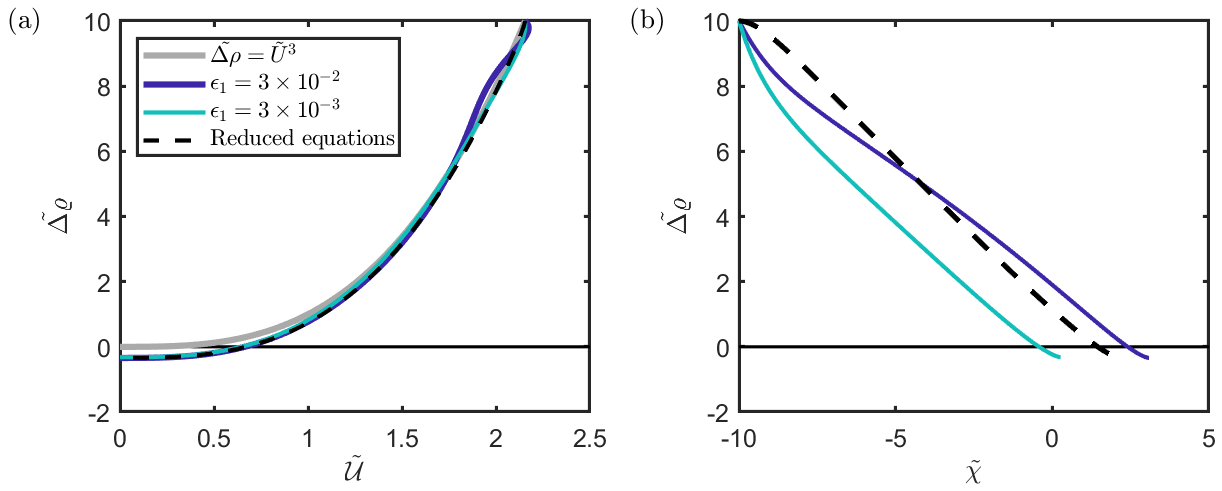
\includegraphics[width = 0.95\textwidth]{Submitted_PRSA/make_plots/plots/supp_fig1.png}
\caption{Numerical solutions of original model equations [(2.30)--(2.33) in the main text] rescaled according to~(3.31)--(3.32) and with $\epsone = 3\times 10^{-2}$ (i.e. as in table 2 of the main text, purple curves) and with $\epsone = 3\times 10^{-3}$ (cyan curves) which are shown in (a) $(\tilde{\U}, \tilde{\p})$ space and (b) $(\tilde{\chi}, \tilde{\p})$ space [$\tilde{\chi}$, $\tilde{\U}$, and $\tilde{\p}$ are a spatial variable, plume velocity, and buoyancy deficit, respectively, and are defined in~\eqref{E:Region4:RescalingChi}--\eqref{E:Region4:RescalingP}]. The black dashed curve indicates the numerical solution of the reduced equations~\eqref{E:Region4:rescaled}, and the grey curve indicates the nullcline $\tilde{\U}^3 = \tilde{\p}$. The solid black line indicates $\tilde{p} = 0$. Each of the solutions here uses a linear draft, $Z_b(X) = X$, with $Q_c = 0.5, X_c = 0.5$ and $\kappa, k_i$ according to the values in table 2 of the main text. The matching conditions~\eqref{E:Region4:far_field1}--\eqref{E:Region4:far_field2} are applied at $\tilde{\chi}_0 = 10$ in both cases, i.e. the solution domain shown is $-\tilde{\chi}_0 < \tilde{\chi} < \tilde{\chi}_t$, where $\tilde{\chi}_t$ is the value of $\tilde{\chi}$ at which the plume velocity reaches zero.}\label{fig:Region4}
\end{figure}

The system~\eqref{E:Region4:rescaled}--\eqref{E:Region4:Rescaled_farfield} must be solved numerically. In figure~\ref{fig:Region4}, we present a comparison between numerical solutions of equations~\eqref{E:Region4:rescaled} and the solutions of the full equations [model equations~(2.30)--(2.33) in the main text rescaled according to~(3.31)--(3.32)]. We see good agreement, with solutions predominantly following the nullcline $\tilde{\p} = \tilde{\U}^3$, before deviating when the rescaled buoyancy deficit $\tilde{\p}$ approaches zero. Eventually, the buoyancy deficit goes negative, indicating that the plume has become negatively buoyant; the plume's upward motion continues for a short distance owing to inertia, before ultimately reaching $\tilde{\U} = 0$, where it terminates. For the purpose of constructing an approximation to the melt rate, it is worth noting that the rescaled buoyancy is approximately linear (figure~\ref{fig:Region4}b); using this, the nullcline solution for $\tilde{\U}$, which holds nearly everywhere in this region, can be approximated by $\tilde{\U} = \tilde{\chi}^{1/3}$. After undoing the rescaling~\eqref{E:Region4:RescalingChi}--\eqref{E:Region4:RescalingP}, this approximate solution reduces to equation (3.37) in the main text. 

%%%%%%%%%%%%%%%%%%%% Melt Rate in Exception Cases %%%%%%%%
\section{Melt Rate Construction in Special Cases}
In this section, we explicity set out our constructed melt rate profiles in the special cases described in \S4 of the main text.

The first special case arises when $\Delta \rho_{\in} - 2 \Pb Z_b'(X_p) < 0$. Our analysis suggests that, in this case, the plume will intrude into the ambient within the pycnocline. Our constructed melt rate takes a linear interpolation across the pycnocline as in the approximation presented in the main text [equation (4.12) therein] that is modified to include zero speed and thermal driving upon exiting:
\begin{equation}\label{E:MeltRate1}
M_{p} = \begin{cases} 
M_{p,1~} \text{~\quad [equation~(4.1)]}  & 0 < X < X_p - N_l \lt,\\
M_{p,2~} \text{~\quad [equation~(4.4)]} & X_p - N_l \lt < X <X_{\text{sep}} ,\\
0  &  X > X_{\text{sep}},\\
\end{cases}
\end{equation}
where $X_{\text{sep}}$ is the value of $X$ at which $M_{p,2} = 0$. \blue{We note that the formulation~\eqref{E:MeltRate1} does not account for the subregion within the pycnocline in which the buoyancy deficit ceases to be $\order{1}$ and the plume velocity reaches zero; this is justified on account of this region having a lengthscale which is $\order{\epsone \delta}$, meaning that it is unimportant on the lengthscale of the entire shelf.}

The second exception case occurs when no physically relevant solution of~(4.7), which describes the `cross-over' point $X^*$ must satisfy, exists. In this case,  the scaled melt rate takes values
\begin{equation}\label{E:MeltRate:AllRegions_noroot}
M_{p} = \begin{cases} 
M_{p,1~} \text{~\quad [equation~(4.1)]}  & 0 < X < X_p - N_l \lt,\\
M_{p,2~} \text{~\quad [equation~(4.4)]} & X_p - N_l \lt < X < X_p + N_l \lt,\\
M_{p,3l~} \text{\quad [equation~(4.8)]} &  X > X_p + N_l \lt.
\end{cases}
\end{equation}
Finally, if the computed termination point $X_c$ does not satisfy $X_c > X^*$, we take $M_p$ as in~\eqref{E:MeltRate:AllRegions_noroot}.

\end{document}